%\documentclass[handout]{ximera}
\documentclass{ximera}

\usepackage{gensymb}
\usepackage{tabularx}
\usepackage{mdframed}
\usepackage{pdfpages}
%\usepackage{chngcntr}

\let\problem\relax
\let\endproblem\relax

\newcommand{\property}[2]{#1#2}




\newtheoremstyle{SlantTheorem}{\topsep}{\fill}%%% space between body and thm
 {\slshape}                      %%% Thm body font
 {}                              %%% Indent amount (empty = no indent)
 {\bfseries\sffamily}            %%% Thm head font
 {}                              %%% Punctuation after thm head
 {3ex}                           %%% Space after thm head
 {\thmname{#1}\thmnumber{ #2}\thmnote{ \bfseries(#3)}} %%% Thm head spec
\theoremstyle{SlantTheorem}
\newtheorem{problem}{Problem}[]

%\counterwithin*{problem}{section}



%%%%%%%%%%%%%%%%%%%%%%%%%%%%Jenny's code%%%%%%%%%%%%%%%%%%%%

%%% Solution environment
%\newenvironment{solution}{
%\ifhandout\setbox0\vbox\bgroup\else
%\begin{trivlist}\item[\hskip \labelsep\small\itshape\bfseries Solution\hspace{2ex}]
%\par\noindent\upshape\small
%\fi}
%{\ifhandout\egroup\else
%\end{trivlist}
%\fi}
%
%
%%% instructorIntro environment
%\ifhandout
%\newenvironment{instructorIntro}[1][false]%
%{%
%\def\givenatend{\boolean{#1}}\ifthenelse{\boolean{#1}}{\begin{trivlist}\item}{\setbox0\vbox\bgroup}{}
%}
%{%
%\ifthenelse{\givenatend}{\end{trivlist}}{\egroup}{}
%}
%\else
%\newenvironment{instructorIntro}[1][false]%
%{%
%  \ifthenelse{\boolean{#1}}{\begin{trivlist}\item[\hskip \labelsep\bfseries Instructor Notes:\hspace{2ex}]}
%{\begin{trivlist}\item[\hskip \labelsep\bfseries Instructor Notes:\hspace{2ex}]}
%{}
%}
%% %% line at the bottom} 
%{\end{trivlist}\par\addvspace{.5ex}\nobreak\noindent\hung} 
%\fi
%
%


\let\instructorNotes\relax
\let\endinstructorNotes\relax
%%% instructorNotes environment
\ifhandout
\newenvironment{instructorNotes}[1][false]%
{%
\def\givenatend{\boolean{#1}}\ifthenelse{\boolean{#1}}{\begin{trivlist}\item}{\setbox0\vbox\bgroup}{}
}
{%
\ifthenelse{\givenatend}{\end{trivlist}}{\egroup}{}
}
\else
\newenvironment{instructorNotes}[1][false]%
{%
  \ifthenelse{\boolean{#1}}{\begin{trivlist}\item[\hskip \labelsep\bfseries {\Large Instructor Notes: \\} \hspace{\textwidth} ]}
{\begin{trivlist}\item[\hskip \labelsep\bfseries {\Large Instructor Notes: \\} \hspace{\textwidth} ]}
{}
}
{\end{trivlist}}
\fi


%% Suggested Timing
\newcommand{\timing}[1]{{\bf Suggested Timing: \hspace{2ex}} #1}




\hypersetup{
    colorlinks=true,       % false: boxed links; true: colored links
    linkcolor=blue,          % color of internal links (change box color with linkbordercolor)
    citecolor=green,        % color of links to bibliography
    filecolor=magenta,      % color of file links
    urlcolor=cyan           % color of external links
}

\title{Playing with Blocks}
\author{Bart Snapp and Brad Findell}

\outcome{Learning outcome goes here.}

\begin{document}
\begin{abstract}
Abstract goes here.  
\end{abstract}
\maketitle

\label{A:B1}
\index{base-ten blocks} 

I always enjoyed blocks quite a bit. Go find yourself
some \textit{base-ten blocks}. Just so that we are all on the same
page, here are the basic blocks:
\begin{image}
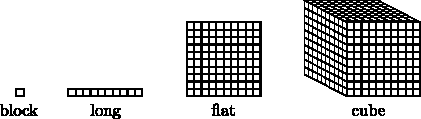
\includegraphics{baseTenBlocks.pdf}
\end{image}

\begin{problem} 
Sketch a model of the number $247$ with base-ten blocks.
\vspace{0.8in}
\end{problem}

\begin{problem}
Oscar modeled the number $15$ in the following way:
\begin{image}
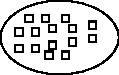
\includegraphics{oscarModel.pdf}
\end{image}
What do you think of his model?  Can you improve upon it?  
\vspace{0.5in}
\end{problem}

\begin{teachingnote}
The issue here is that the place-value system is not modeled. When
working with base-ten blocks, we will demand that the place value
system is always modeled.  We want to do this with all algorithms.
\end{teachingnote}

\begin{problem}
Many problems involving subtraction can be considered one of the
following types: take-away, comparison, and missing addend.  Write a
``word problem'' illustrating each of these types.
\end{problem}

\begin{problem} 
Here is a standard subtraction algorithm:\index{subtraction algorithm!standard}
\[
\normalfont
\begin{tabular}{@{}r@{}r@{}r@{}r@{}}
&   & 8 &  \\
& 8 & $\not{\hspace{-.2ex}9}$ & $\hspace{.3ex}\leftexp{1}2$\\
$-$ & 3 & 7 & 8\\ \hline
& 5 & 1 & 4
\end{tabular}
\]
Use base-ten blocks to model this algorithm.  Which type of subtraction are you using?  
\end{problem}

\newpage
\begin{problem}
Oscar uses base-ten blocks to model subtraction.  
\begin{image}
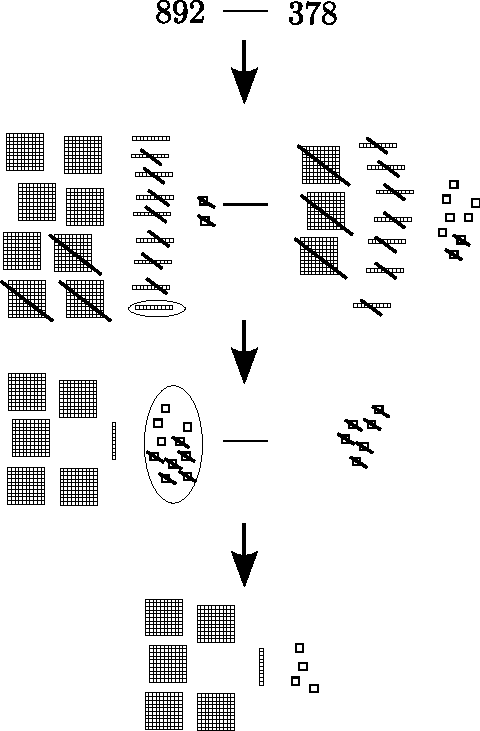
\includegraphics{oscarSub.pdf}
\end{image}
Can you explain what is going on?  Which type of subtraction is Oscar using?  
\end{problem}

\begin{problem} Create a ``new'' subtraction algorithm based on Oscar's model.
\end{problem}

\newpage
\begin{problem}
Here is an example of a standard addition algorithm:
\[
\normalfont
\begin{tabular}{@{}r@{}}
11~~\\
892\\
+398\\ \hline
1290
\end{tabular}
\]
Model this algorithm with base-ten blocks.
\end{problem}

\end{document}
